
%%%%%%%%%%%%%%%%%%%%%%%%%%%%%%%%%%%%%%%%%%%%%%%%%%%%%%%%%%%%%%%%%%%%%%%%%%%%%%%%
%% ************************************************************************** %%
%% *                                Settings                                * %%
%% ************************************************************************** %%
%%%%%%%%%%%%%%%%%%%%%%%%%%%%%%%%%%%%%%%%%%%%%%%%%%%%%%%%%%%%%%%%%%%%%%%%%%%%%%%%
\documentclass{tron}

\loadglsentries{gls}
\glsaddall
\addbibresource{reference}
\usepackage{xcolor}  % Coloured text etc.
% fancy note style
% STYLE NOTES : v2.0
% additional fancy boxes
\usepackage[framemethod=TikZ]{mdframed}
%\usepackage{amsthm}

% gray color indicates [OPTIONAL READING]

%%%%%%%%%%%%%%%%%%%%%%%%%%%%%%
%Note
\newenvironment{note}[3][]{%
	\ifstrempty{#1}%
	{\mdfsetup{%
	frametitle={%
	\tikz[baseline=(current bounding box.east),outer sep=0pt]
	\node[anchor=east,rectangle,fill=#2]
	{\strut Note};}}
	}%
	{\mdfsetup{%
	frametitle={%
	\tikz[baseline=(current bounding box.east),outer sep=0pt]
	\node[anchor=east,rectangle,fill=#2]
	{\strut #1};}}%
	}%
	\mdfsetup{innertopmargin=0pt,skipabove=5pt,linecolor=#2,%
		linewidth=2pt,topline=true,%
		frametitleaboveskip=\dimexpr-\ht\strutbox\relax,
		backgroundcolor={white!90!#2}}
	\begin{mdframed}[]\relax%
	\label{#3}}{\end{mdframed}
}
\Crefname{note}{Note}{notes}

\newcommand{\createnoteenv}[6]{
	\refstepcounter{#6}%
	\ifstrempty{#1}%
	{\mdfsetup{%
	frametitle={%
	\tikz[baseline=(current bounding box.east),outer sep=0pt]
	\node[anchor=east,rectangle,fill=#3]
	{\strut #4~#5};}}
	}%
	{
		\mdfsetup{%
			frametitle={%
				\tikz[baseline=(current bounding box.east),outer sep=0pt]
				\node[anchor=east,rectangle,fill=#3]
				{\strut #4~#5:~#1};
			}
		}%
	}%
	\mdfsetup{innertopmargin=0pt,skipabove=5pt,linecolor=#3,%
	linewidth=2pt,topline=true,%
	frametitleaboveskip=\dimexpr-\ht\strutbox\relax,
	backgroundcolor={white!90!#3}}
	\begin{mdframed}[]\relax%
	\label{#2}
}

%%%%%%%%%%%%%%%%%%%%%%%%%%%%%%
%Definition
\newcounter{definition}[section] \setcounter{definition}{0}
\renewcommand{\thedefinition}{\arabic{section}.\arabic{definition}}
\newenvironment{definition}[2][]{%
	\createnoteenv{#1}{#2}{blue!40}{Definition}{\thedefinition}{definition}%
}{\end{mdframed}}
\newenvironment{definition*}[2][]{%
	\createnoteenv{#1}{#2}{gray!40}{Definition}{\thedefinition}{definition}%
}{\end{mdframed}}
\Crefname{definition}{Definition}{definitions}


%%%%%%%%%%%%%%%%%%%%%%%%%%%%%%
%theoremrem
\newcounter{theorem}[section] \setcounter{theorem}{0}
\renewcommand{\thetheorem}{\arabic{section}.\arabic{theorem}}
\newenvironment{theorem}[2][]{%
	\createnoteenv{#1}{#2}{cyan!40}{Theorem}{\thetheorem}{theorem}%
}{\end{mdframed}}
\newenvironment{theorem*}[2][]{%
	\createnoteenv{#1}{#2}{gray!40}{Theorem}{\thetheorem}{theorem}%
}{\end{mdframed}}
\Crefname{theorem}{Theorem}{theorems}

%%%%%%%%%%%%%%%%%%%%%%%%%%%%%%
%Proof
\newcounter{proof}[section]\setcounter{proof}{0}
\renewcommand{\theproof}{\arabic{section}.\arabic{proof}}
\newenvironment{proof}[2][]{%
	\createnoteenv{#1}{#2}{red!20}{Proof}{\theproof}{proof}%
}{\end{mdframed}}
\newenvironment{proof*}[2][]{%
	\createnoteenv{#1}{#2}{gray!40}{Proof}{\theproof}{proof}%
}{\end{mdframed}}
\Crefname{proof}{Proof}{proofs}


%%%%%%%%%%%%%%%%%%%%%%%%%%%%%%
%Alert
\newcounter{alert}[section]\setcounter{alert}{0}
\renewcommand{\thealert}{\arabic{section}.\arabic{alert}}
\newenvironment{alert}[2][]{%
	\createnoteenv{#1}{#2}{red!80}{Alert}{\thealert}{alert}%
}{\end{mdframed}}
\newenvironment{alert*}[2][]{%
	\createnoteenv{#1}{#2}{gray!40}{Alert}{\thealert}{alert}%
}{\end{mdframed}}
\Crefname{alert}{Alert}{alerts}

%%%%%%%%%%%%%%%%%%%%%%%%%%%%%%
%Answer
\newcounter{answer}[section]\setcounter{answer}{0}
\renewcommand{\theanswer}{\arabic{section}.\arabic{answer}}
\newenvironment{answer}[2][]{%
	\createnoteenv{#1}{#2}{orange!60}{Answer}{\theanswer}{answer}%
}{\end{mdframed}}
\newenvironment{answer*}[2][]{%
	\createnoteenv{#1}{#2}{gray!40}{Answer}{\theanswer}{answer}%
}{\end{mdframed}}
\Crefname{answer}{Answer}{answers}

%%%%%%%%%%%%%%%%%%%%%%%%%%%%%%
%Remark
\newcounter{remark}[section]\setcounter{remark}{0}
\renewcommand{\theremark}{\arabic{section}.\arabic{remark}}
\newenvironment{remark}[2][]{%
	\createnoteenv{#1}{#2}{orange!40}{Remark}{\theremark}{remark}%
}{\end{mdframed}}
\newenvironment{remark*}[2][]{%
	\createnoteenv{#1}{#2}{gray!40}{Remark}{\theremark}{remark}%
}{\end{mdframed}}
\Crefname{remark}{Remark}{remarks}


%%%%%%%%%%%%%%%%%%%%%%%%%%%%%%%
%%Example
%\newcounter{example}[section]\setcounter{example}{0}
%\renewcommand{\theexample}{\arabic{section}.\arabic{example}}
%\newenvironment{example}[2][]{%
%	\createnoteenv{#1}{#2}{blue!40!cyan!20}{Example}{\theexample}{example}%
%}{\end{mdframed}}
%\newenvironment{example*}[2][]{%
%	\createnoteenv{#1}{#2}{gray!40}{Example}{\theexample}{example}%
%}{\end{mdframed}}

%%%%%%%%%%%%%%%%%%%%%%%%%%%%%%
%Algorithm
\newcounter{algo}[section]\setcounter{algo}{0}
\renewcommand{\thealgo}{\arabic{algo}.\arabic{algo}}
\newenvironment{algo}[2][]{%
	\createnoteenv{#1}{#2}{yellow!90!brown!60}{Algorithm}{\thealgo}{algo}%
}{\end{mdframed}}
\newenvironment{algo*}[2][]{%
	\createnoteenv{#1}{#2}{gray!40}{Algorithm}{\thealgo}{algo}%
}{\end{mdframed}}
\Crefname{algo}{Algorithm}{algos}

%%%%%%%%%%%%%%%%%%%%%%%%%%%%%%
% CS480 - Exercise
%\setlength{\parskip}{1cm}
%\setlength{\parindent}{1cm}

%\tikzstyle{titregris} =
%[draw=gray,fill=white, shading = exersicetitle, %
%text=gray, rectangle, rounded corners, right,minimum height=.3cm]
%\pgfdeclarehorizontalshading{exersicebackground}{100bp}
%{color(0bp)=(green!40); color(100bp)=(black!5)}
%\pgfdeclarehorizontalshading{exersicetitle}{100bp}
%{color(0bp)=(red!40);color(100bp)=(black!5)}
%\newcounter{exercise}
%\renewcommand*\theexercise{exercice \textbf{Exercice}~n\arabic{exercise}}
%\makeatletter
%\def\mdf@@exercisepoints{}%new mdframed key:
%\define@key{mdf}{exercisepoints}{%
%\def\mdf@@exercisepoints{#1}
%}
%
%\mdfdefinestyle{theoremstyle}{%
%outerlinewidth=0.01em,linecolor=black,middlelinewidth=0.5pt,%
%frametitlerule=true,roundcorner=2pt,%
%apptotikzsetting={\tikzset{mfframetitlebackground/.append style={%
%shade,left color=white, right color=blue!20}}},
%frametitlerulecolor=black,innertopmargin=1\baselineskip,%green!60,
%innerbottommargin=0.5\baselineskip,
%frametitlerulewidth=0.1pt,
%innertopmargin=0.7\topskip,skipabove={\dimexpr0.2\baselineskip+0.1\topskip\relax},
%frametitleaboveskip=1pt,
%frametitlebelowskip=1pt
%}
%\mdtheorem[style=theoremstyle]{exercise}{\textbf{Exercise}}

\newcounter{exercise}[section]\setcounter{exercise}{0}
\renewcommand{\theexercise}{\arabic{exercise}}
\newenvironment{exercise}[2][]{%
	\createnoteenv{#1}{#2}{gray!40}{Exercise}{\theexercise}{exercise}%
}{\end{mdframed}}
\newenvironment{exercise*}[2][]{%
	\createnoteenv{#1}{#2}{gray!40}{Exercise}{\theexercise}{exercise}%
}{\end{mdframed}}

\Crefname{exercise}{Exercise}{exercises}


%%%%%%%%%%%%%%%%%%%%%%%%%%%%%%
%Examples
% {

%     \section{Theorem and lemma examples with title}
%     \begin{theorem}[Pythagoras' theorem]{theorem:pythagoras}
%     In a right triangle, the square of the hypotenuse is equal to the sum of the squares of the catheti.
%     \[a^2+b^2=c^2\]
%     \end{theorem}
%     In mathematics, the Pythagorean theorem, also known as Pythagoras' theorem (see theorem \ref{theorem:pythagoras}), is a relation in Euclidean geometry among the three sides of a right triangle.
%     
%     \begin{definition}[B\'ezout's identity]{def:bezout}
%     Let $a$ and $b$ be nonzero integers and let $d$ be their greatest common divisor. Then there exist integers $x$ and $y$ such that:
%     \[ax+by=d\]
%     \end{definition}
%     This is a reference to Bezout's lemma \ref{def:bezout}
%     
%     
%     \section{Theorem and proof examples without title}
%     
%     \begin{theorem}[]{theorem:theorem1}
%     There exist two irrational numbers $x$, $y$ such that $x^y$ is rational.
%     \end{theorem}
%     
%     \begin{proof}[]{proof:proof1}
%     If $x=y=\sqrt{2}$ is an example, then we are done; otherwise $\sqrt{2}^{\sqrt{2}}$ is irrational, in which case taking $x=\sqrt{2}^{\sqrt{2}}$ and $y=\sqrt{2}$ gives us:
%     \[\bigg(\sqrt{2}^{\sqrt{2}}\bigg)^{\sqrt{2}}=\sqrt{2}^{\sqrt{2}\sqrt{2}}=\sqrt{2}^{2}=2.\]
%     \end{proof}
%
%     \begin{alert}[]{alert:alert1}
%     If $x=y=\sqrt{2}$ is an example, then we are done; otherwise $\sqrt{2}^{\sqrt{2}}$ is irrational, in which case taking $x=\sqrt{2}^{\sqrt{2}}$ and $y=\sqrt{2}$ gives us:
%     \[\bigg(\sqrt{2}^{\sqrt{2}}\bigg)^{\sqrt{2}}=\sqrt{2}^{\sqrt{2}\sqrt{2}}=\sqrt{2}^{2}=2.\]
%     \end{alert}
%     
%     \begin{remark}[]{alert:alert1}
%     If $x=y=\sqrt{2}$ is an example, then we are done; otherwise $\sqrt{2}^{\sqrt{2}}$ is irrational, in which case taking $x=\sqrt{2}^{\sqrt{2}}$ and $y=\sqrt{2}$ gives us:
%     \[\bigg(\sqrt{2}^{\sqrt{2}}\bigg)^{\sqrt{2}}=\sqrt{2}^{\sqrt{2}\sqrt{2}}=\sqrt{2}^{2}=2.\]
%     \end{remark}
%     
%     
%          \begin{exercise}[]{alert:alert1}
%     If $x=y=\sqrt{2}$ is an example, then we are done; otherwise $\sqrt{2}^{\sqrt{2}}$ is irrational, in which case taking $x=\sqrt{2}^{\sqrt{2}}$ and $y=\sqrt{2}$ gives us:
%     \[\bigg(\sqrt{2}^{\sqrt{2}}\bigg)^{\sqrt{2}}=\sqrt{2}^{\sqrt{2}\sqrt{2}}=\sqrt{2}^{2}=2.\]
%     \end{exercise}
%     
%     \begin{algo}[]{algorithm:alert1}
%     If $x=y=\sqrt{2}$ is an example, then we are done; otherwise $\sqrt{2}^{\sqrt{2}}$ is irrational, in which case taking $x=\sqrt{2}^{\sqrt{2}}$ and $y=\sqrt{2}$ gives us:
%     \[\bigg(\sqrt{2}^{\sqrt{2}}\bigg)^{\sqrt{2}}=\sqrt{2}^{\sqrt{2}\sqrt{2}}=\sqrt{2}^{2}=2.\]
%     \end{algo}
%     
%     \begin{note}[Goal]{pink}{note:goal}
%     If $x=y=\sqrt{2}$ is an example, then we are done; otherwise $\sqrt{2}^{\sqrt{2}}$ is irrational, in which case taking $x=\sqrt{2}^{\sqrt{2}}$ and $y=\sqrt{2}$ gives us:
%     \[\bigg(\sqrt{2}^{\sqrt{2}}\bigg)^{\sqrt{2}}=\sqrt{2}^{\sqrt{2}\sqrt{2}}=\sqrt{2}^{2}=2.\]
%     \end{note}

% }
%\usepackage{lipsum}                     % Dummytext
\usepackage{xargs}                      % Use more than one optional parameter in a new commands
\usepackage[colorinlistoftodos,prependcaption,textsize=normalsize]{todonotes}
%
\newcommandx{\unsure}[2][1=]{\todo[linecolor=red,backgroundcolor=red!25,bordercolor=red,#1]{#2}}
\newcommandx{\change}[2][1=]{\todo[linecolor=blue,backgroundcolor=blue!25,bordercolor=blue,#1]{#2}}
\newcommandx{\info}[2][1=]{\todo[linecolor=OliveGreen,backgroundcolor=OliveGreen!25,bordercolor=OliveGreen,#1]{#2}}
\newcommandx{\improvement}[2][1=]{\todo[linecolor=Plum,backgroundcolor=Plum!25,bordercolor=Plum,#1]{#2}}
\newcommandx{\thiswillnotshow}[2][1=]{\todo[disable,#1]{#2}}
%
\preto\printlistoftodos{
    \listoftodos[Todo List]
}

% EXAMPLES:
    % \todo[inline]{The original todo note withouth changed colours.\newline Here's another line.}
    % \lipsum[11]\unsure{Is this correct?}\unsure{I'm unsure about also!}
    % \lipsum[11]\change{Change this!}
    % \lipsum[11]\info{This can help me in chapter seven!}
    % \lipsum[11]\improvement{This really needs to be improved!\newline\newline What was I thinking?!}
    % \lipsum[11]
    % \thiswillnotshow{This is hidden since option `disable' is chosen!}
    % \improvement[inline]{The following section needs to be rewritten!}
    % \lipsum[11]
    % \newpage
    % \listoftodos[Notes]
%%%  Equation Condition
\newenvironment{eqconditions}
  {\par\vspace{\abovedisplayskip}\noindent\begin{tabular}{>{$}l<{$} @{${}={}$} l}}
  {\end{tabular}\par\vspace{\belowdisplayskip}}
\newenvironment{eqconditions*}
  {\noindent\begin{tabular}{>{$}l<{$} @{${}={}$} l}}
  {\end{tabular}}
%%% introduce 4th depth with \paragraph command
\usepackage{titlesec}
\setcounter{secnumdepth}{4}
\titleformat{\paragraph}
{\normalfont\normalsize\bfseries}{\theparagraph}{1em}{}
\titlespacing*{\paragraph}
{0pt}{3.25ex plus 1ex minus .2ex}{1.5ex plus .2ex}

%%% enumeration reference
% constraint
\newlist{constraint-list}{enumerate}{1}
\setlist[constraint-list,1]{leftmargin=*, label= \Roman*}
\creflabelformat{Constraint}{#2#1#3}
\crefname{constraint-listi}{Constraint}{position}
% criteria
\newlist{criteria-list}{enumerate}{1}
\setlist[criteria-list,1]{leftmargin=*, label= \Roman*}
\creflabelformat{Criterion}{#2#1#3}
\crefname{criteria-listi}{Criterion}{position}
% property
\newlist{property-list}{enumerate}{1}
\setlist[property-list,1]{leftmargin=*, label= \Roman*}
\creflabelformat{Property}{#2#1#3}
\crefname{property-listi}{Property}{position}
% assumption
\newlist{assumption-list}{enumerate}{1}
\setlist[assumption-list,1]{leftmargin=*, label= \Roman*}
\creflabelformat{Assumption}{#2#1#3}
\crefname{assumption-listi}{Assumption}{position}

% custom math command
\newcommand{\unit}[1]{\left[\si{#1}\right]}

% additional math packages
\usepackage{physics}
\usepackage{cancel}

% TODO Flags
\newcommand\TODO[1]{{\textcolor{red}{\textbf{#1}}}}
\newcommand\COMMENT[1]{\hl{#1}}

% Custom Format
% \usepackage{float}
% \usepackage[table]{xcolor}
% \usepackage{soul}
\usepackage{multirow}
\usepackage{caption} 
\captionsetup[table]{skip=3pt}
\captionsetup[figure]{skip=0pt}
\titlespacing*{\section}
{0pt}{10pt}{3pt}
\titlespacing*{\subsection}
{0pt}{8pt}{3pt}
\titlespacing*{\subsubsection}
{0pt}{8pt}{3pt}
%hide the highlight box
\hypersetup{
    colorlinks,
    linkcolor={black!50!black},
    citecolor={black!50!blue},
    urlcolor={black!80!black}
}%hide the highlight box

% table formatting
% \setlength{\arrayrulewidth}{1mm}
% \setlength{\tabcolsep}{18pt}
% \renewcommand{\arraystretch}{2.5}
\usepackage{array}
\newcolumntype{C}[1]{>{\centering\let\newline\\\arraybackslash\hspace{0pt}}m{#1}}

% custom math symbol
%% CS 480 %%
\newcommand{\bm}[1]{\mathbf{#1}}
%%%%%%%%%%%%
\newcommand{\RR}{\mathds{R}}
\newcommand{\Id}{\mathbb{I}}
\newcommand{\NN}{\mathds{N}}
\newcommand{\sign}{\mathop{\mathrm{sign}}}
\newcommand{\diag}{\mathop{\mathrm{diag}}}
\newcommand{\argmin}{\mathop{\mathrm{argmin}}}
\newcommand{\zero}{\mathbf{0}}
\newcommand{\one}{\mathbf{1}}
\newcommand{\av}{\mathbf{a}}
\newcommand{\bv}{\mathbf{b}}
\newcommand{\sv}{\mathbf{s}}
\newcommand{\Xv}{\mathbf{X}}
\newcommand{\Yv}{\mathbf{Y}}
\newcommand{\wv}{\mathbf{w}}
\newcommand{\xv}{\mathbf{x}}
\newcommand{\yv}{\mathbf{y}}
\newcommand{\zv}{\mathbf{z}}
\newcommand{\uv}{\mathbf{u}}
\newcommand{\rv}{\mathbf{r}}
\newcommand{\inner}[2]{\langle #1, #2 \rangle}
\newcommand{\red}[1]{{\color{red}#1}}
\newcommand{\blue}[1]{{\color{blue}#1}}
\newcommand{\magenta}[1]{{\color{magenta}#1}}


\newcommand{\ea}{{et al.}\xspace}
\newcommand{\eg}{{e.g.}\xspace}
\newcommand{\ie}{{i.e.}\xspace}
\newcommand{\iid}{{i.i.d.}\xspace}
\newcommand{\cf}{{cf.}\xspace}
\newcommand{\wrt}{{w.r.t.}\xspace}
\newcommand{\aka}{{a.k.a.}\xspace}
\newcommand{\etc}{{etc.}\xspace}
\newcommand{\sgm}{\mathsf{sgm}}
\newcommand{\Dc}{\mathcal{D}}
\newcommand{\ans}[1]{{\textcolor{orange}{\textsf{Ans}: #1}}}



\usepackage{float}
% extra mod
\newcommand{\mref}[1]{\underline{\textbf{\hypersetup{linkcolor=orange}\Cref{#1}\hypersetup{linkcolor=blue}}}}


\newcommand{\apx}{\text{approx}}

%%%%%%%%%%%%%%%%%%%%%%%%%%%%%%%%%%%%%%%%%%%%%%%%%%%%%%%%%%%%%%%%%%%%%%%%%%%%%%%%
% Make sure the following block contains the correct information               %
%%%%%%%%%%%%%%%%%%%%%%%%%%%%%%%%%%%%%%%%%%%%%%%%%%%%%%%%%%%%%%%%%%%%%%%%%%%%%%%%
\reporttitle{ECE 488 - Project 5 \& 6}
% \selfstudy % comment this line if this is not a self study report 
% \employername{Employer Name}
% \employerstreetaddress{Employer Address}
% \employerlocation{City, Provice, Country}
\university{University of Waterloo}
\faculty{Faculty of Engineering}%Faculty of Engineering
\department{Department of Electrical and Computer Engineering}%Department of Systems Design Engineering
\groupnumber{1}
\authornameA{Jianxiang (Jack) Xu}
\studentnumberA{20658861}
\reportdate{\today}
%\confidential{1} % comment this line if this is not a confidential report
%\authorstreetaddress{##}
%\authorlocation{##}
%\authorpostalcode{##}
\useheader % comment this line if no need for header
%%%%%%%%%%%%%%%%%%%%%%%%%%%%%%%%%%%%%%%%%%%%%%%%%%%%%%%%%%%%%%%%%%%%%%%%%%%%%%%%
% end of information block...                                                  %
%%%%%%%%%%%%%%%%%%%%%%%%%%%%%%%%%%%%%%%%%%%%%%%%%%%%%%%%%%%%%%%%%%%%%%%%%%%%%%%%

\begin{document}
%%%%%%%%%%%%%%%%%%%%%%%%%%%%%%%%%%%%%%%%%%%%%%%%%%%%%%%%%%%%%%%%%%%%%%%%%%%%%%%%
%% ************************************************************************** %%
%% *                               Title Page                               * %%
%% ************************************************************************** %%
%%%%%%%%%%%%%%%%%%%%%%%%%%%%%%%%%%%%%%%%%%%%%%%%%%%%%%%%%%%%%%%%%%%%%%%%%%%%%%%%
\maketitle
%%%%%%%%%%%%%%%%%%%%%%%%%%%%%%%%%%%%%%%%%%%%%%%%%%%%%%%%%%%%%%%%%%%%%%%%%%%%%%%%
%% ************************************************************************** %%
%% *                           Table of Contents                            * %%
%% ************************************************************************** %%
%%%%%%%%%%%%%%%%%%%%%%%%%%%%%%%%%%%%%%%%%%%%%%%%%%%%%%%%%%%%%%%%%%%%%%%%%%%%%%%%
 \tableofcontents
%%%%%%%%%%%%%%%%%%%%%%%%%%%%%%%%%%%%%%%%%%%%%%%%%%%%%%%%%%%%%%%%%%%%%%%%%%%%%%%%
%% ************************************************************************** %%
%% *                            List of Figures                             * %%
%% ************************************************************************** %%
%%%%%%%%%%%%%%%%%%%%%%%%%%%%%%%%%%%%%%%%%%%%%%%%%%%%%%%%%%%%%%%%%%%%%%%%%%%%%%%%
% \listoffigures
%%%%%%%%%%%%%%%%%%%%%%%%%%%%%%%%%%%%%%%%%%%%%%%%%%%%%%%%%%%%%%%%%%%%%%%%%%%%%%%%
%% ************************************************************************** %%
%% *                             List of Tables                             * %%
%% ************************************************************************** %%
%%%%%%%%%%%%%%%%%%%%%%%%%%%%%%%%%%%%%%%%%%%%%%%%%%%%%%%%%%%%%%%%%%%%%%%%%%%%%%%%
% \listoftables
%%%%%%%%%%%%%%%%%%%%%%%%%%%%%%%%%%%%%%%%%%%%%%%%%%%%%%%%%%%%%%%%%%%%%%%%%%%%%%%%
%% ************************************************************************** %%
%% *                              MAIN BODY                                 * %%
%% ************************************************************************** %%
%%%%%%%%%%%%%%%%%%%%%%%%%%%%%%%%%%%%%%%%%%%%%%%%%%%%%%%%%%%%%%
\clearpage
\pagenumbering{arabic}
\setcounter{page}{1}
\setlength{\parskip}{5pt}
\newpage

%%%%%%%%%%%%%%%%%%%%%%%%%%%%%%%%%%%
%%%%% Intro.  %%%%%%
%%%%%%%%%%%%%%%%%%%%%%%%%%%%%%%%%%%

%%%%%%%%%%%%%%%%
%%%%% Ex 5 %%%%%
%%%%%%%%%%%%%%%%
\section{Problem P5: Decentralized MIMO control of the aiming system}
%\vspace{5pt}
Notation clarification: $(row, column)$: $(1,1)=r_w \rightarrow w$, $(2,1)=r_w \rightarrow \theta$, $(1,2)=r_{\theta} \rightarrow w$, and $(2,2)=r_{\theta} \rightarrow \theta$.

% --- ANS (a) --- %
\subsection{(a) Justification from MIMO Bode Plot of $P_3(s)$ \label{ans:P5-a}}

As we may observed in the \Cref{fig:p5:P3:bode} below, we may observe the magnitude gain for both $(1,2)$ and $(2,1)$ are below $0\unit{dB}$, and the phase margin is $0 \unit{deg}$. This is a great indication that the cross-channel interference is minimal. For the DC gain (steady-state), the diagonal terms $(1,1)$ and $(2,2)$ of the plant dominant the entire system. Specifically, the (1,1) term indicates that the force input $u_1 = F$ dominants the effect of base displacement $y_1 = w$, and has negligible effect on rod angle $y_2 = \theta$ as $(2, 1)$ bode suggested. Similarly, the (2,2) term indicates the torque input $u_2 = \tau$ dominants the effect of the rod angle $y_2 = \theta$. 

\begin{figure}[H]
	\centering
	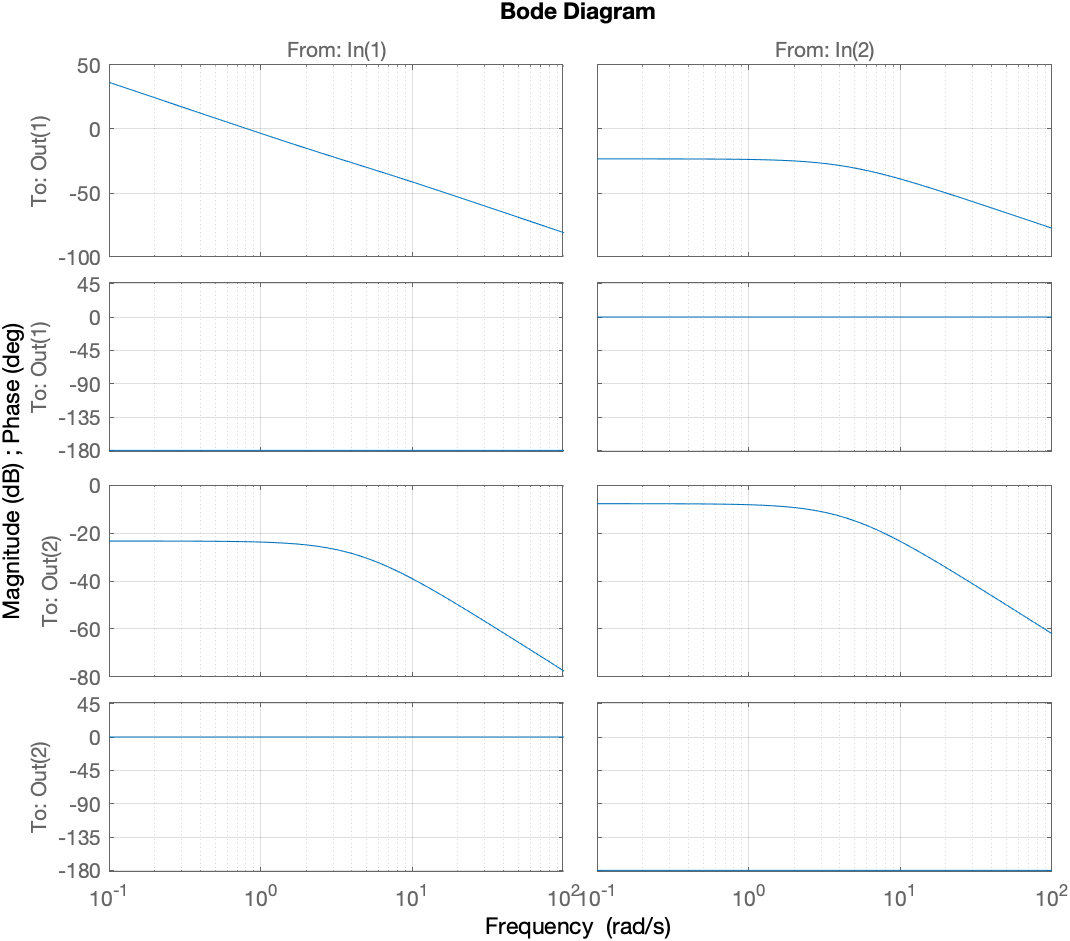
\includegraphics[height=400px]{../matlab/output/p5/P3_bode_plot}
	\caption{Bode Plot of $P_3(s)$}
	\label{fig:p5:P3:bode}
\end{figure}

Hence, we can control the base position using the force input and control the rod angle using the torque input. Consequently, we can apply decentralized design strategy to this particular MIMO system. 

\clearpage
% --- ANS (b) --- %
\subsection{(b) Derivation of $P_{3, \apx}(s)$ \label{ans:P5-b}}
Recall the actual $P_3(s)$, we have previously found there is little effect on the steady-state from the cross-channel. We may deal the system as a decentralized system.
\begin{equation}
	P_{3}(s) = 
	\begin{bmatrix}
		-\frac{0.8889\,(s+3.834)\,(s-3.834)}{s^2\,(s-4.427)\,(s+4.427)} & \frac{-1.3333\,s^2}{s^2 \, (s-4.427)\,(s+4.427)} \\
		-\frac{-1.3333}{(s-4.427)\,(s+4.427)} & \frac{8.0}{(s-4.427)\,(s+4.427)}
	\end{bmatrix}
	\label{eqn:p5:p3-actual}
\end{equation}

However, instead of blindly ignoring the off-diagonal terms within $P_3(s)$, we can design an approximated plant by isolating the system:

Firstly, from the perspective of the force input, we can treat the entire system as whole:
\begin{align}
	F &= (m + M) \ddot{w} \\
	\textbf{Laplace Tranform + T.S. Expansion}  & \Rightarrow \, F(s) = (m + M)(s^2 W(s) + s \cancelto{0}{\dot{w}(0)} + \cancelto{0}{w(0)})  \\
	& \Rightarrow \, P_{3,\apx,11} = \frac{W(s)}{F(s)} = \frac{1}{(m + M) \, s^2}
\end{align}

Lastly, from the perspective of the torque input, we can treat the position base is fixed, and only compute the effect of the rod:
\begin{align}
	\tau + mg \frac{L}{2}\, \sin \theta &= J \ddot{\theta}\\
	\textbf{Laplace Tranform + T.S. Expansion}  & \Rightarrow \, T(s) = \frac{mL^2}{3}\,(s^2 \Theta(s)) - mg \frac{L}{2} \Theta(s) \\
	& \Rightarrow \, P_{3,\apx , 22} = \frac{\Theta(s)}{T(s)} = \frac{6}{ 2 mL^2\, s^2 - 3 mgL}
\end{align}

As a result, we can form the approximated plant $P_{3, \apx}(s)$ as:
\begin{align}
	P_{3, \apx}(s) = 
	\begin{bmatrix}
		\frac{1}{(m + M) \, s^2} & 0 \\
		0 & \frac{6}{ 2 mL^2\, s^2 - 3 mgL} 
	\end{bmatrix}
	= 
	\begin{bmatrix}
		\frac{0.66667}{s^2} & 0 \\
		0 & \frac{6.0}{(s-3.834)(s+3.834)}
	\end{bmatrix}	
	\label{eqn:p5:p3-approx}
\end{align}

To further ensure the integrity of the approximated plant, we may plot the bode plot of the plant as well. As we may see from \Cref{fig:p5:P3_aug:bode} below, the diagonal channels indeed appear to be similar to the original bode plot in \Cref{fig:p5:P3:bode}. 
\begin{figure}[H]
	\centering
	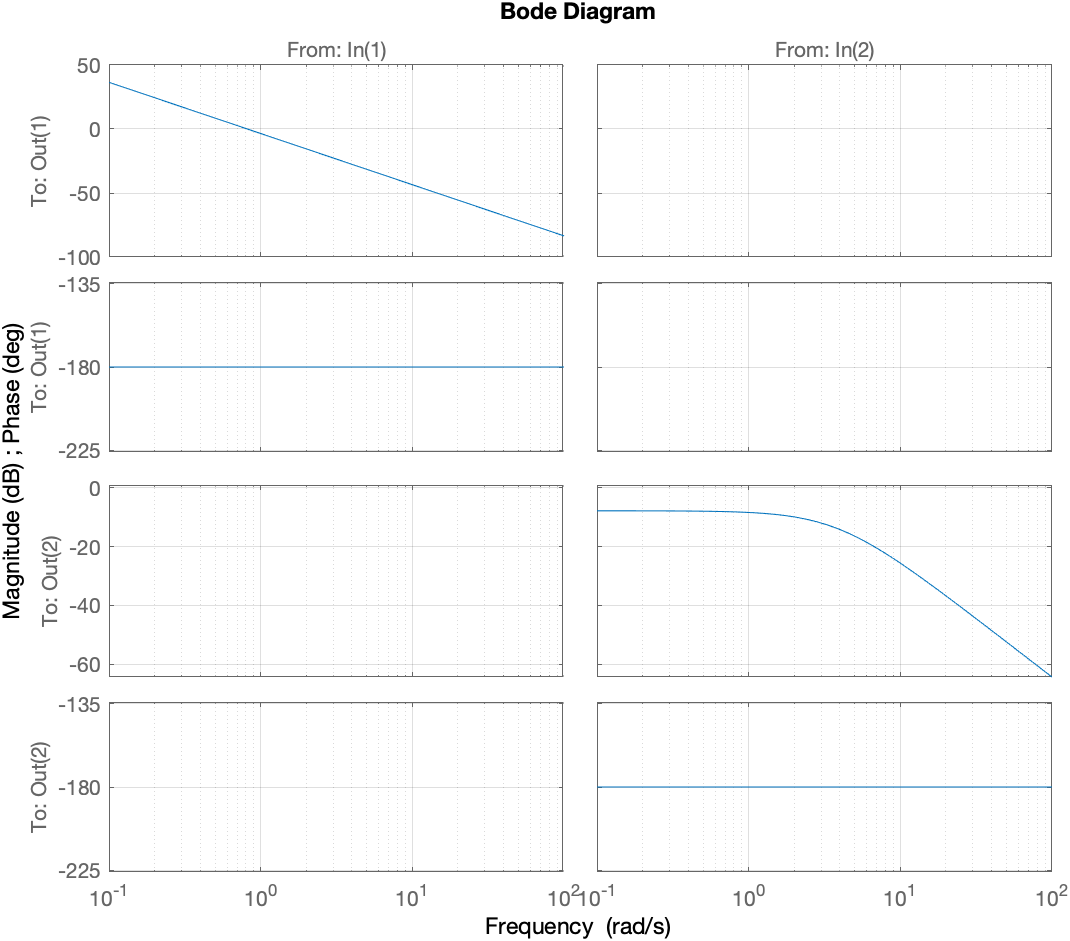
\includegraphics[height=400px]{../matlab/output/p5/P3_aug_bode_plot}
	\caption{Bode Plot of $P_{3, \apx}(s)$}
	\label{fig:p5:P3_aug:bode}
\end{figure}

\clearpage
% --- ANS (c) --- %
\subsection{(c) Design 1-DOF SISO Controller $C_{11}(s)$ for the (1,1) entry of $P_{3, \apx}(s)$ \label{ans:P5-c}}
Three design specifications are imposed:
\begin{spec-list}
	\item Closed-loop stable \label{spec:stable}
	\item Perfect steady-state tracking \label{spec:track}
	\item PM $\geq 50^{\circ}$ \label{spec:pm}
\end{spec-list}

As we may observe from $(1,1)$ entry in the bode plot from \Cref{fig:p5:P3_aug:bode}, the phase margin is $0^{\circ}$. As a result, we need a lead filter to pull up the phase margin to satisfy \Cref{spec:pm}. Since, we have double integrator in the $P_{3, \apx, 11}(s)$ plant, it naturally satisfy the perfect steady-state tracking \Cref{spec:track}. As a result, the closed loop system should be stable. 

Using the \verb|'sisotool'|, we may manually find the suitable controller quickly, as seen in \Cref{fig:p5:P3_aug11:siso}.
\begin{figure}[H]
	\centering
	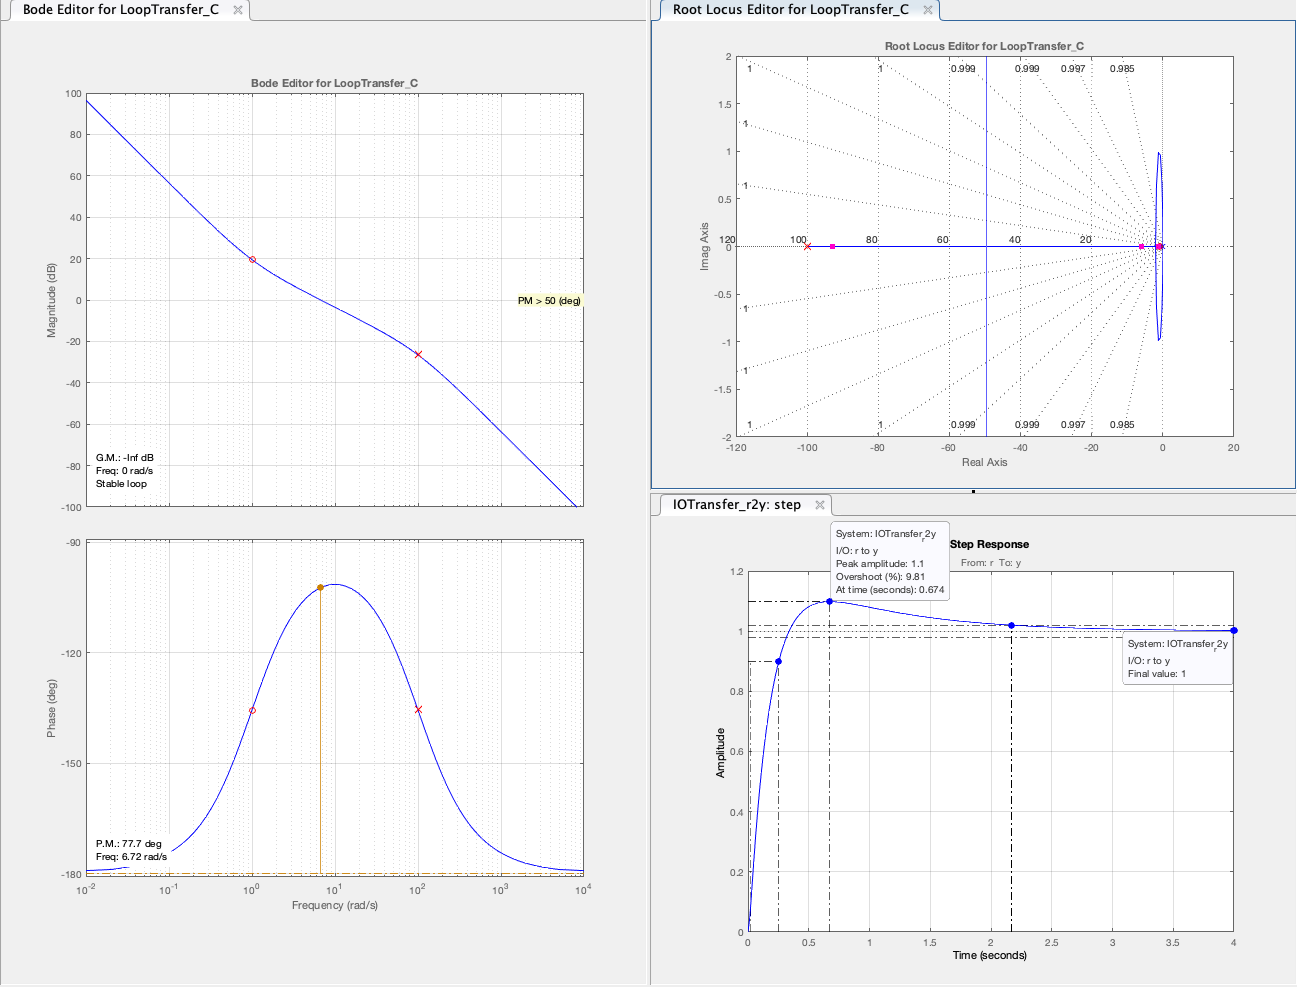
\includegraphics[height=350px]{../matlab/misc/sisotool_P3_aug_11.png}
	\caption{SISO design tool of closed-loop controller design for $P_{3, \apx, 11}(s)$}
	\label{fig:p5:P3_aug11:siso}
\end{figure}

As a result, the SISO controller we designed for $P_{3, \apx, 11}(s)$ is: 
\begin{align}
	C_{11}(s) = \frac{1000 \, (s + 1)}{(s + 100)}	
	\label{eqn:p5:c11}
\end{align}

We may also plot the final plot of bode diagram, root locus, and the step response similar to the \verb|'sisotool'|:
\begin{figure}[H]
	\centering
	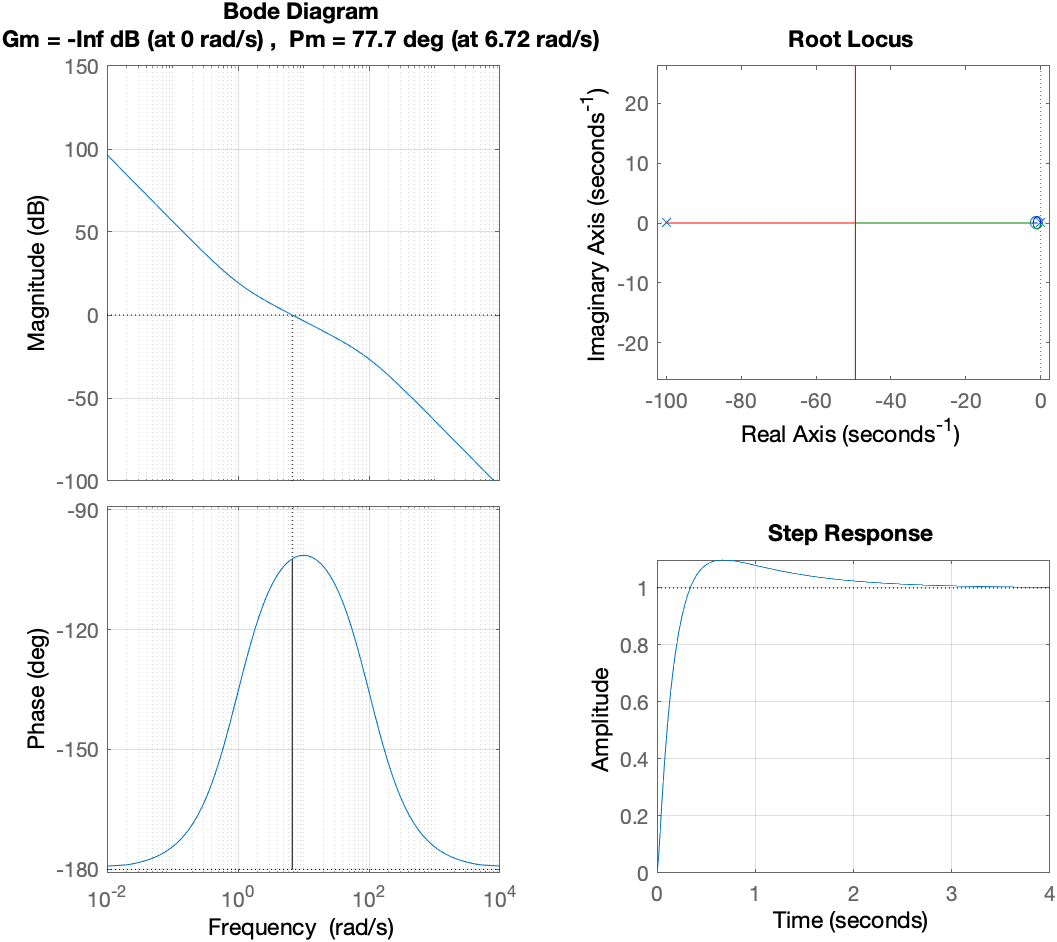
\includegraphics[height=400px]{../matlab/output/p5/siso_plot_Ideal(1,1)}
	\caption{Final SISO plot of closed-loop controller design for $P_{3, \apx, 11}(s)$}
	\label{fig:p5:P3_aug11:siso-final}
\end{figure}


\clearpage
% --- ANS (d) --- %
\subsection{(d) Design 1-DOF SISO Controller $C_{22}(s)$ for the (2,2) entry of $P_{3, \apx}(s)$ \label{ans:P5-d}}
Similarly, as we may observe from $(2,2)$ entry in the bode plot from \Cref{fig:p5:P3_aug:bode}, the phase margin is $0^{\circ}$. As a result, we need a lead filter to pull up the phase margin to satisfy \Cref{spec:pm}. In this case, we do not have any integrator in the $P_{3, \apx, 22}(s)$ plant, hence, there is a need to include an integrator inside the controller to achieve the perfect steady-state tracking \Cref{spec:track}. 

To note, there exists a RHP pole in the plant. In order to make the closed loop system stable (\Cref{spec:stable}), we need to introduce a LHP zero between the stable and unstable pole to pull the closed-loop pole to the LHP.

Using the \verb|'sisotool'|, we may manually find the suitable controller quickly, as seen in \Cref{fig:p5:P3_aug22:siso}. Firstly, adding an integrator in the controller, and introduce a LHP zero at $s=-3$ and adjust the gain to make the closed-loop poles back into the OLHP. Lastly, adding the lead filter to make the phase margin above the \Cref{spec:pm}.

\begin{figure}[H]
	\centering
	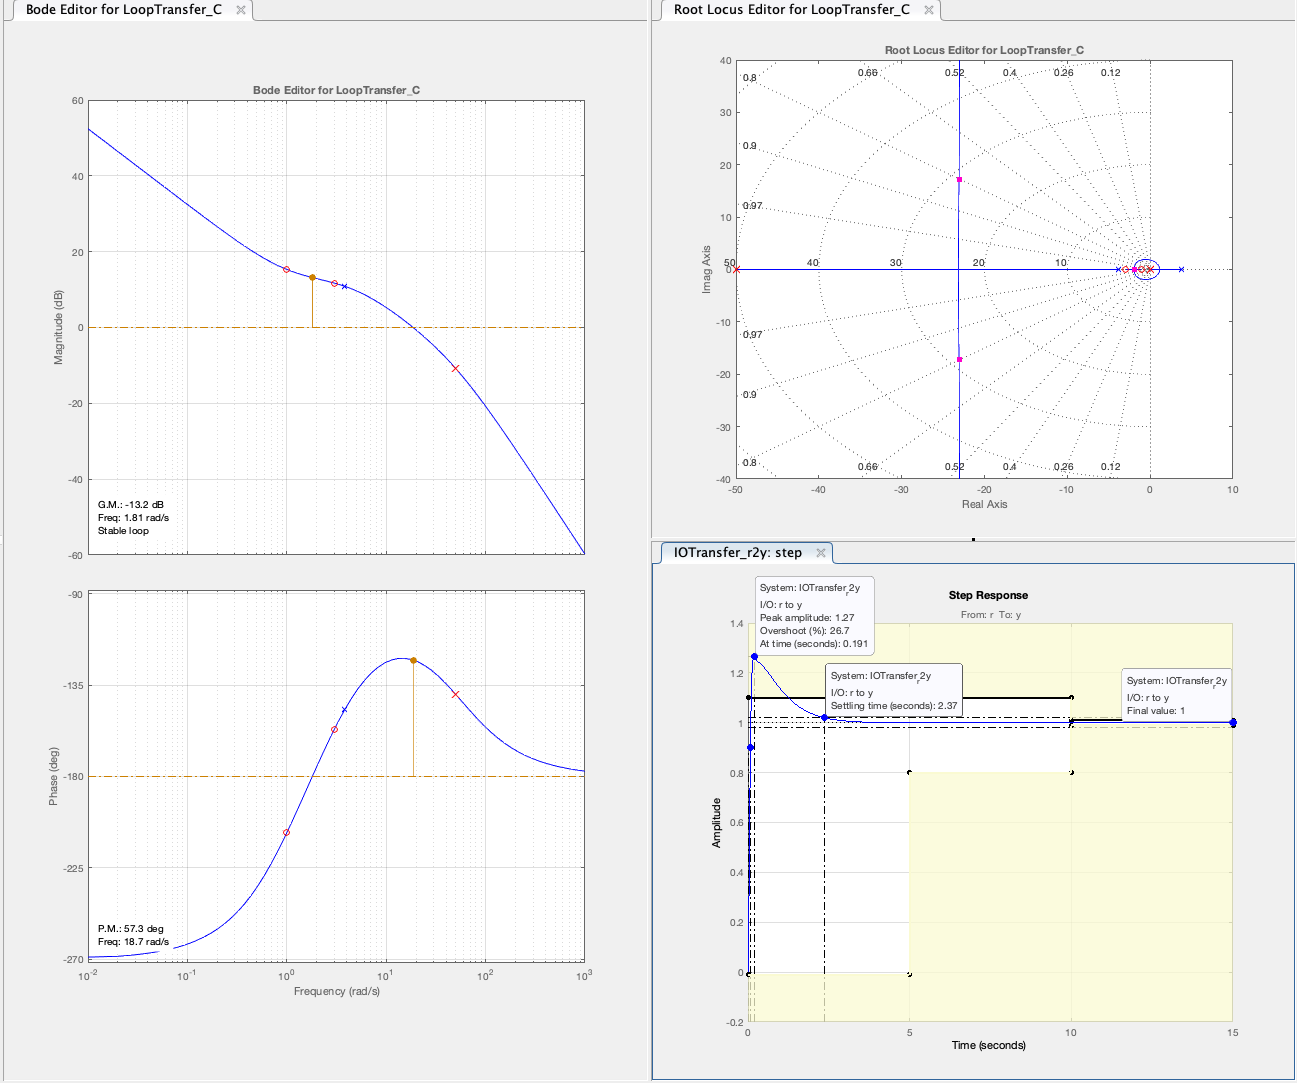
\includegraphics[height=350px]{../matlab/misc/sisotool_P3_aug_22.png}
	\caption{SISO design tool of closed-loop controller design for $P_{3, \apx, 22}(s)$}
	\label{fig:p5:P3_aug22:siso}
\end{figure}

As a result, the SISO controller we designed for $P_{3, \apx, 22}(s)$ is: 
\begin{align}
	C_{11}(s) = \frac{170.54 \, (s+1) (s+3)}{(s+50) s}	
	\label{eqn:p5:c22}
\end{align}

We may also plot the final plot of bode diagram, root locus, and the step response similar to the \verb|'sisotool'|:
\begin{figure}[H]
	\centering
	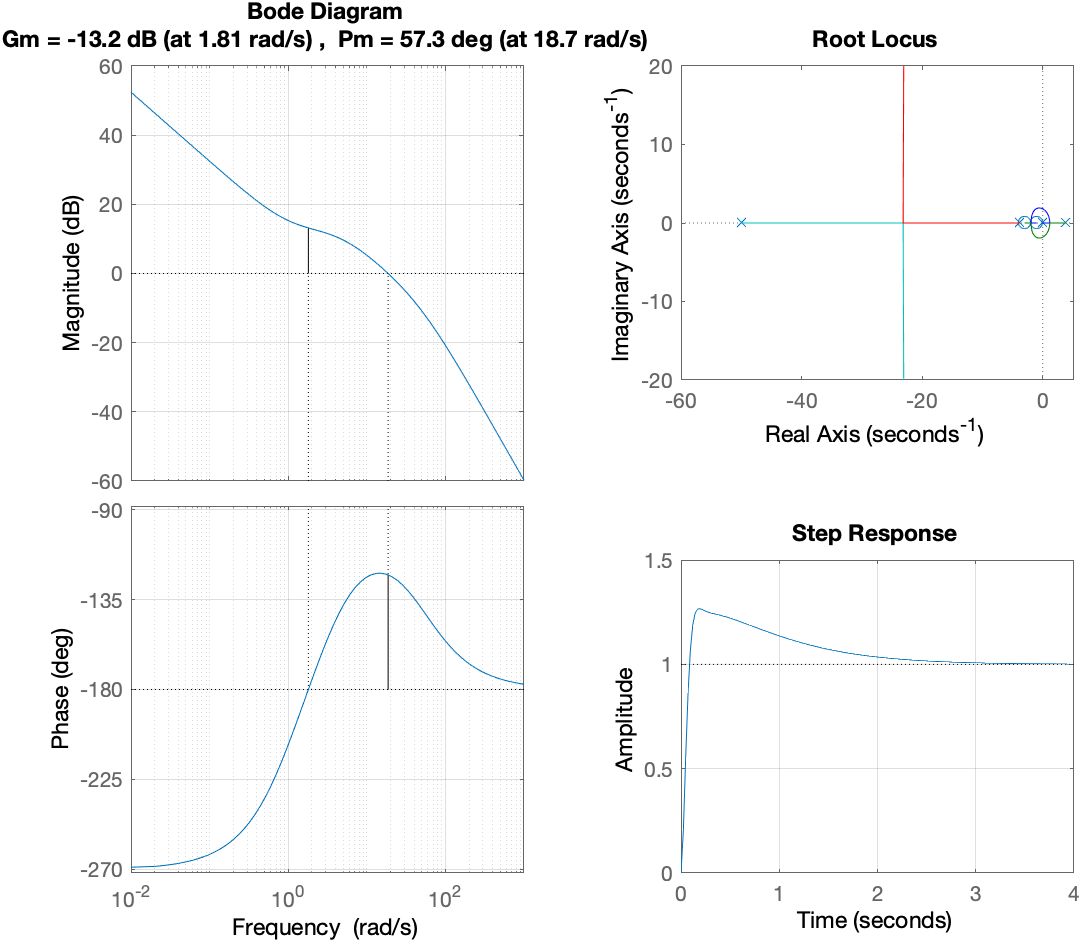
\includegraphics[height=400px]{../matlab/output/p5/siso_plot_Ideal(2,2)}
	\caption{Final SISO plot of closed-loop controller design for $P_{3, \apx, 22}(s)$}
	\label{fig:p5:P3_aug22:siso-final}
\end{figure}

\clearpage
% --- ANS (e) --- %
\subsection{(e) Analyze the designed controller $C_{3}(s)$ \label{ans:P5-e}}
From \Cref{ans:P5-c} and \Cref{ans:P5-d}, we may obtain the final controller designed for the approximated plant $P_{3, \apx}$:

\begin{align}
	C_{3}(s) = 
	\begin{bmatrix}
		\frac{1000 \, (s + 1)}{(s + 100)} & 0 \\
		0 &  \frac{170.54 \, (s+1) (s+3)}{(s+50) s}	
	\end{bmatrix}
	\label{eqn:p5:c3}
\end{align}

Let's apply this final controller with the approximated plant $P_{3, \apx}(s)$ it designed from. We may obtain the step response graph as shown in \Cref{fig:p5:P3_aug:step-response} below and both transient and steady-state performance as shown in \Cref{table:p5:perf:ideal} below.

\begin{figure}[H]
	\centering
	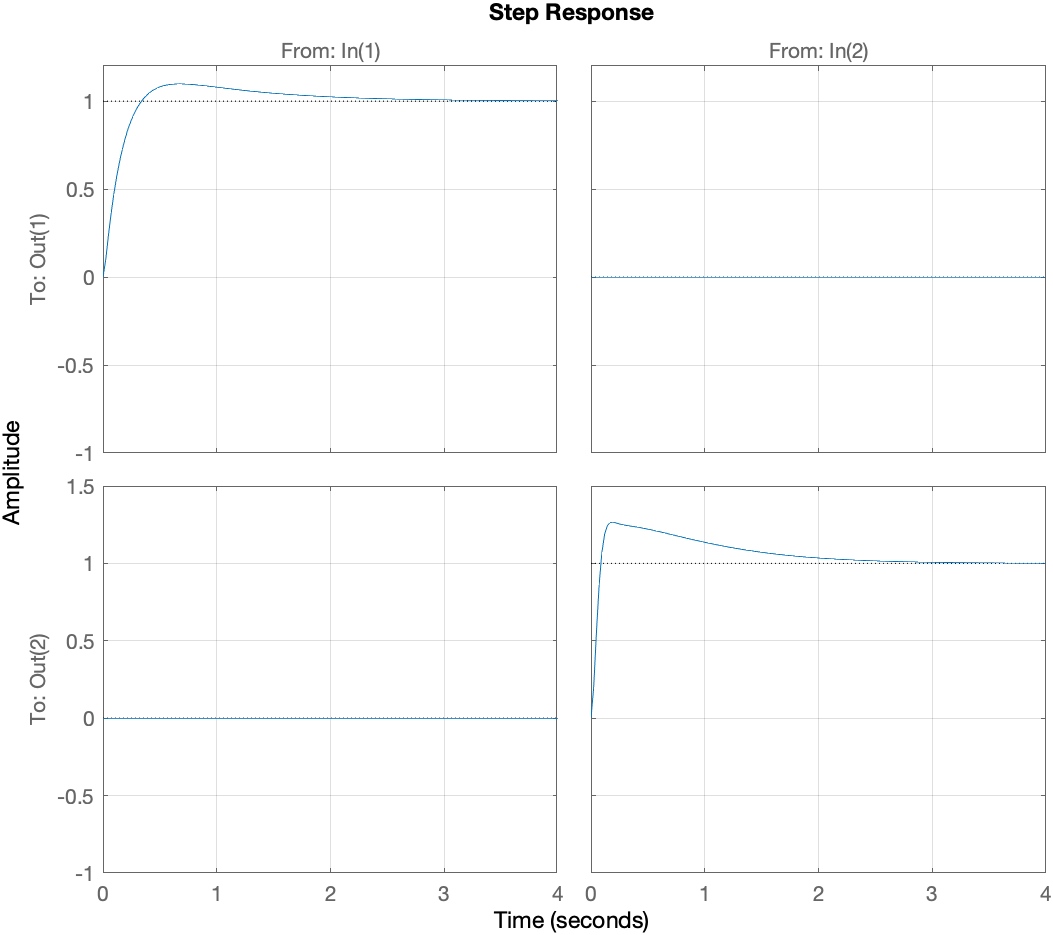
\includegraphics[height=350px]{../matlab/output/p5/Ideal_step_response}
	\caption{Ideal step response with the approximated plant $P_{3, \apx}(s)$}
	\label{fig:p5:P3_aug:step-response}
\end{figure}

\begin{table}[h!]
  \begin{center}
    \caption{Ideal Performance Summary ($C_{3}(s)$ with $P_{3, \apx}(s)$)}
    \label{table:p5:perf:ideal}
		\begin{tabular}{llllllll}
		& $t_{rise}$ & $t_{settling}$ & $t_{peak}$ & $y_{peak}$ & $y_{ss}$ & OS\% & US\% \\ 
		\hline 
		(1,1) & 0.2298 & 2.1687 & 0.67103 & 1.0981 & 1.0037 & 9.8058 & 0 \\ 
		(1,2) & 0 & 0 & 0 & 0 & 0 & $\infty$ & 0 \\ 
		(2,1) & 0 & 0 & 0 & 0 & 0 & $\infty$ & 0 \\ 
		(2,2) & 0.064222 & 2.3662 & 0.19172 & 1.2666 & 1.003 & 26.6601 & 0 \\ 
		\hline 
		\end{tabular}
  \end{center}
\end{table}

Similarly, let's apply this final controller with the actual plant $P_{3}(s)$ it designed from. We may obtain the step response graph as shown in \Cref{fig:p5:P3:step-response} below and both transient and steady-state performance as shown in \Cref{table:p5:perf:actual} below.

\begin{figure}[H]
	\centering
	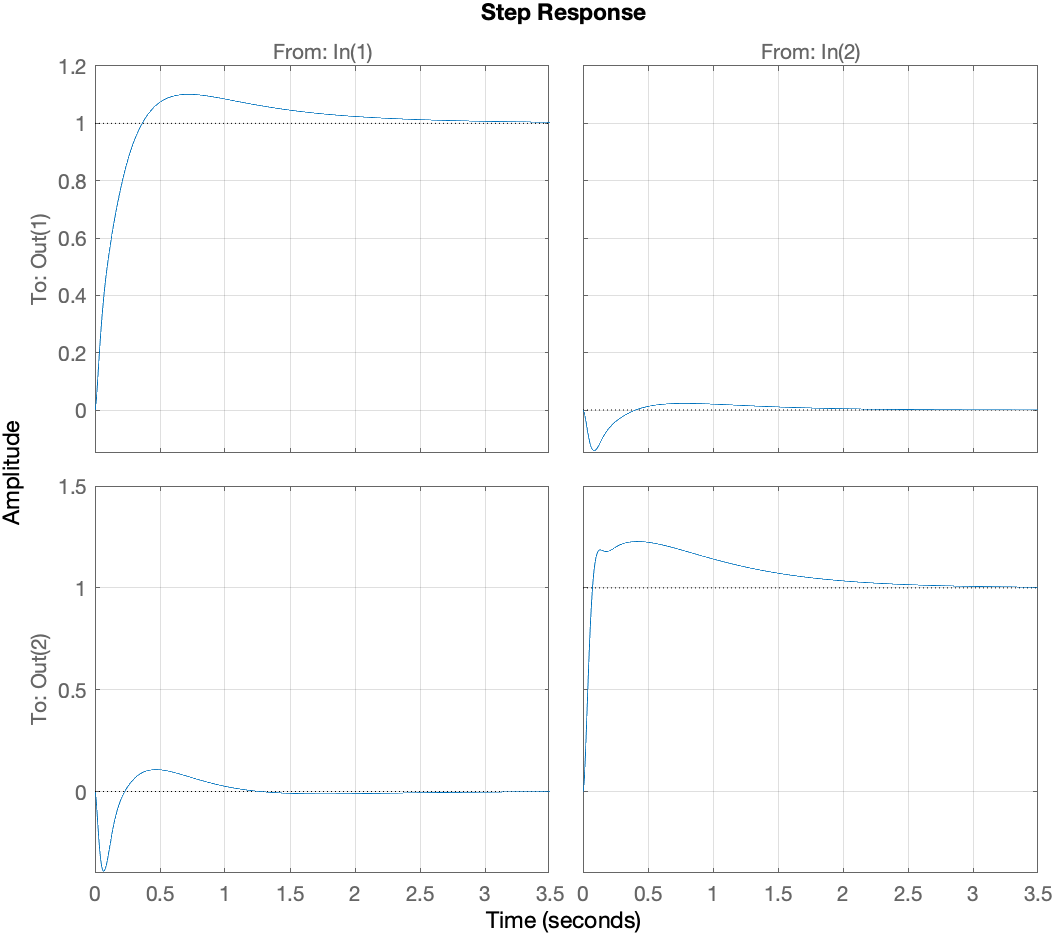
\includegraphics[height=350px]{../matlab/output/p5/Actual_step_response}
	\caption{Actual step response with the actual plant $P_{3}(s)$}
	\label{fig:p5:P3:step-response}
\end{figure}

\begin{table}[h!]
  \begin{center}
    \caption{Actual Performance Summary ($C_{3}(s)$ with $P_{3}(s)$)}
    \label{table:p5:perf:actual}
		\begin{tabular}{llllllll}
		& $t_{rise}$ & $t_{settling}$ & $t_{peak}$ & $y_{peak}$ & $y_{ss}$ & $OS\%$ & $US\%$ \\ 
		\hline 
		(1,1) & 0.2506 & 2.143 & 0.71721 & 1.1012 & 1.0044 & 10.1206 & 0 \\ 
		(1,2) & 2.1704e-13 & 2.2418 & 0.085915 & 0.14246 & 0.00015909 & 131127080892444.7 & 21200873797753.34 \\ 
		(2,1) & 3.933e-13 & 2.305 & 0.067238 & 0.39121 & -0.0014772 & 36100623416931.88 & 9911777297481.107 \\ 
		(2,2) & 0.049924 & 2.3456 & 0.41837 & 1.2272 & 1.0038 & 22.7219 & 0 \\ 
		\hline 
		\end{tabular}
  \end{center}
\end{table}


\subsubsection{Assuming the SISO loops from parts (c) and (d) are stable, do you necessarily expect the MIMO closed-loop system to be stable?}
%• Assuming the SISO loops from parts (c) and (d) are stable, do you necessarily expect the MIMO closed-loop system to be stable? Explain your reasoning, and determine whether or not the MIMO system is stable.
As per discussion when justifying the decentralization strategy in \Cref{ans:P5-a}, we can neglect the coupling effect from the cross-channels. As \Cref{fig:p5:P3_aug:bode} suggested, the approximation plant exhibits similar bode characteristics as the original plant. As a result, as long as we give a reasonable GM and PM when designing the controller for the approximated plant $P_{3, \apx}(s)$, we do expect the MIMO likely to be closed-loop stable. But, there is no guarantee that the MIMO closed-loop system in the end to be stable, since the controller was designed neglecting the coupling effects, and a large gain in the controller could possibly excite the coupling term and make the system unstable.

In our controller designed above, the closed-loop system appear to be stable for both the SISO (decentralized MIMO) and actual MIMO system with a unit step input, as both ideal response in \Cref{fig:p5:P3_aug:step-response} and actual response in \Cref{fig:p5:P3:step-response} shown above.

\subsubsection{Assuming the MIMO closed-loop system is stable, is there a guarantee of perfect steady-state tracking for step references?}
%• Assuming the MIMO closed-loop system is stable, is there a guarantee of perfect steady-state tracking for step references? Explain your reasoning, and use Matlab to determine the actual steady-state performance.
Assuming the MIMO closed-loop system is stable, there is no guarantee of 100\% perfect steady-state tracking. Depending on the coupling term, the coupling term may have some effect on the final steady-state. 

In our particular scenario, the actual steady-state performance is close to perfect (as stated in \Cref{table:p5:perf:actual}): 1.0044 and 1.0038 for diagonal terms, and 0.00016 and -0.0015 for the cross-channel terms. The actual steady-state performance is extremely close to the expectation in \Cref{table:p5:perf:ideal}. As a result, the controller we designed is a great controller in terms of steady-state performance with about $<2.5 \unit{s}$ settling time.

\subsubsection{Assuming the MIMO closed-loop system is stable, is there a guarantee that the step response transients will be identical to the step response transients of the individual SISO feedback loops from parts (c) and (d)?}
%• Assuming the MIMO closed-loop system is stable, is there a guarantee that the step response transients will be identical to the step response transients of the individual SISO feedback loops from parts (c) and (d)? Explain your reasoning and use Matlab to determine the actual transient performance.
There is no guarantee that the step response transients would be identical to the step response transients of the individual SISO feedback loops. Since the coupling term would bring some transient impacts to the system, unless there is no coupling effects in the original plant in the first place. 

As we may see from the transient performance tabulated in \Cref{table:p5:perf:actual} and \Cref{table:p5:perf:ideal}, and the step response graph in \Cref{fig:p5:P3:step-response} and \Cref{fig:p5:P3_aug:step-response} for the actual system and approximated system respectively, we can see there are quite difference in terms of transient performance (including rising time, settling time, peak time, peak, overshoot percentage and undershoot percentage. From the step response graph, we can see undershoot and overshoot effects in transient for coupling channels, which was expected to have no or little effect originally. In addition, there is a wobbling effect in the $(2,2)$ entry of the step response. Hence, we can conclude the transient performance would not be identical to the individual SISO feedback, as long as there exists cross-channeling effects originally. 

(We will see and further discuss about these effects visually in the simulation section (\Cref{ans:P5-f}) below).

\clearpage
% --- ANS (f) --- %
\subsection{(f) [Optional] Simulation \label{ans:P5-f}}
Firstly, let's fixed the rod angle, and try to move the base without changing the rod angle.

\begin{figure}[H]
	\centering
	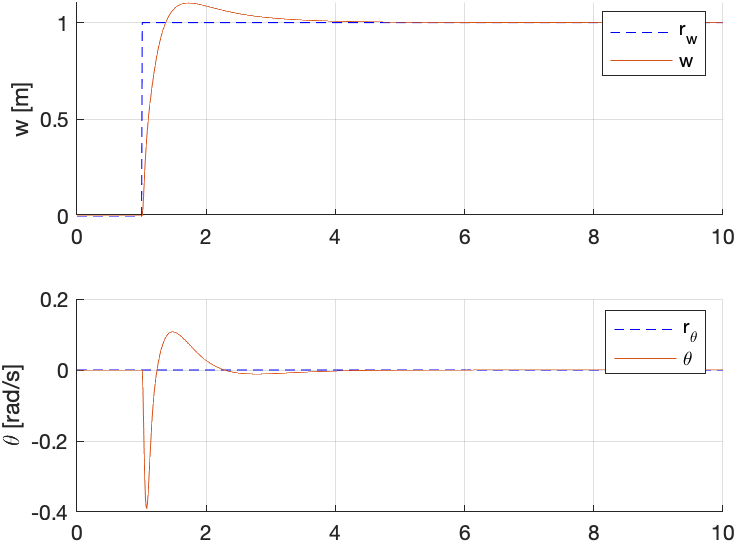
\includegraphics[height=250px]{../matlab/output/p5/square_response_actual-fixed_theta}
	\caption{System response for a step input of base position $r_{w}=1\unit{m}$ with fixed rod angle $r_{theta}=0$}
	\label{fig:p5:P3_aug:sim:fixe-theta}
\end{figure}
\begin{figure}[H]
	\centering
	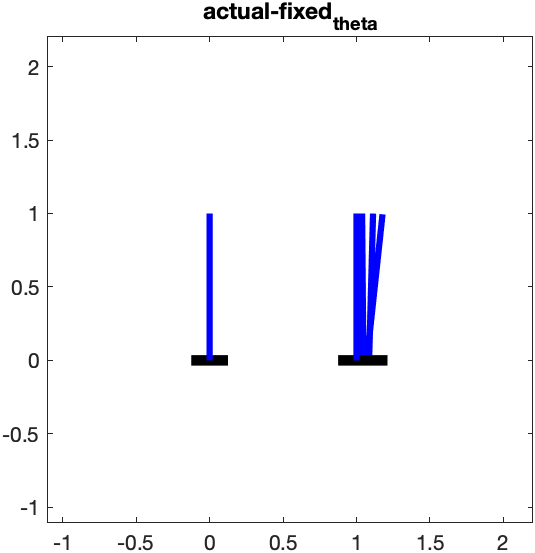
\includegraphics[height=200px]{../matlab/output/p5/mimo_sim_actual-fixed_theta}
	\caption{Simulation of the actual plant with the controller designed (fixed rod angle $r_{theta}=0\unit{rad}$)}
	\label{fig:p5:P3_aug:sim:fixe-theta}
\end{figure}

As we have discussed, we observed the undershoot and overshoot in the actual plant due to the ignorance of cross-channelling effects when designing the controller. This causes a bad transient performance, but the steady-state of the system looks pretty decent. The coupling effect from the base position to the rod angular position is quite significant, and observable in the simulation plot in \Cref{fig:p5:P3_aug:sim:fixe-theta}.

\clearpage
Now, let's fixed the base position, and try to rotate the rod angle without changing the base position.
\begin{figure}[H]
	\centering
	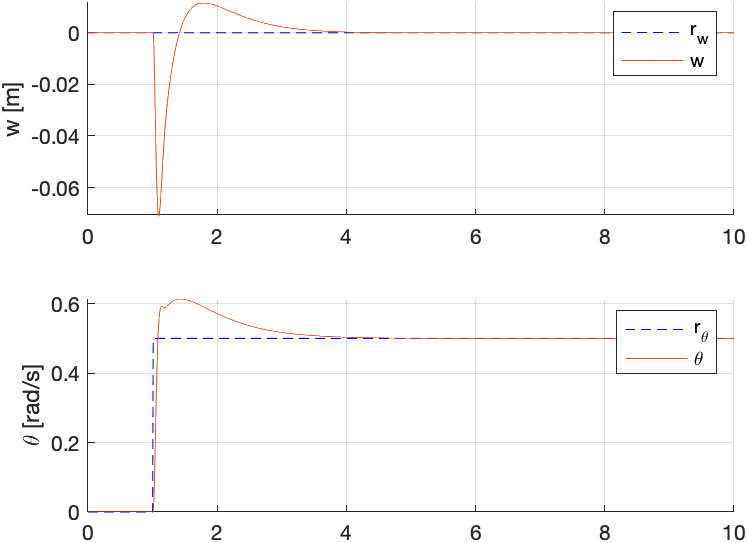
\includegraphics[height=250px]{../matlab/output/p5/square_response_actual-fixed_w}
	\caption{System response for a step input of rod angle $r_{\theta}=0.5\unit{rad}$ with fixed base position $r_{w}=0\unit{m}$}
	\label{fig:p5:P3_aug:sim:fixe-w}
\end{figure}
\begin{figure}[H]
	\centering
	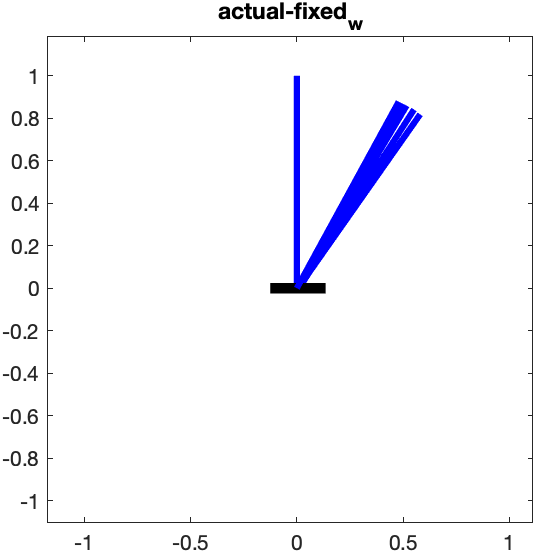
\includegraphics[height=200px]{../matlab/output/p5/mimo_sim_actual-fixed_w}
	\caption{Simulation of the actual plant with the controller designed (fixed base position $r_{w}=0\unit{m}$)}
	\label{fig:p5:P3_aug:sim:fixe-w}
\end{figure}
Similarly, we observed the undershoot and overshoot in the actual plant due to the ignorance of cross-channelling effects when designing the controller. The system indeed reaches a perfect steady-state, despite bad transient performance. To note, this transient effect is almost negligible, hence, we may conclude that the rod angle position has little coupling effect of the base position in this setup (as suggest by \Cref{fig:p5:P3_aug:sim:fixe-w}).

\clearpage
Finally, let's combine both step input.
\begin{figure}[H]
	\centering
	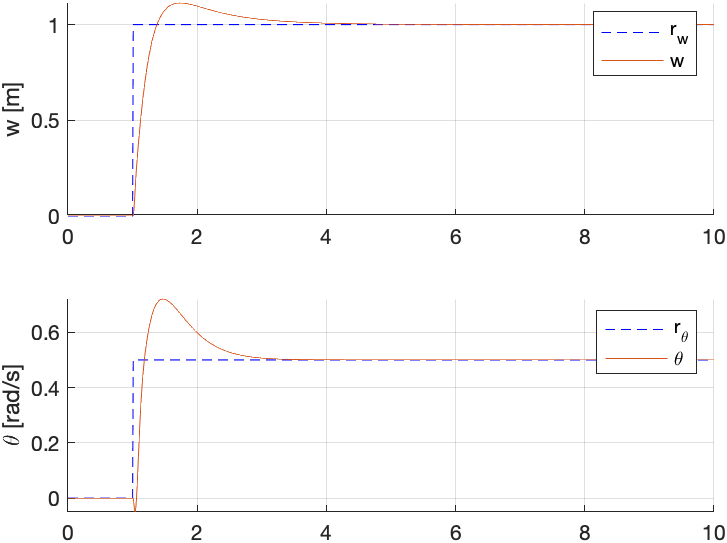
\includegraphics[height=250px]{../matlab/output/p5/square_response_actual-both}
	\caption{System response for a step input of rod angle $r_{\theta}=0.5\unit{rad}$ with a step input of base position $r_{w}=1\unit{m}$}
	\label{fig:p5:P3_aug:sim:both}
\end{figure}
\begin{figure}[H]
	\centering
	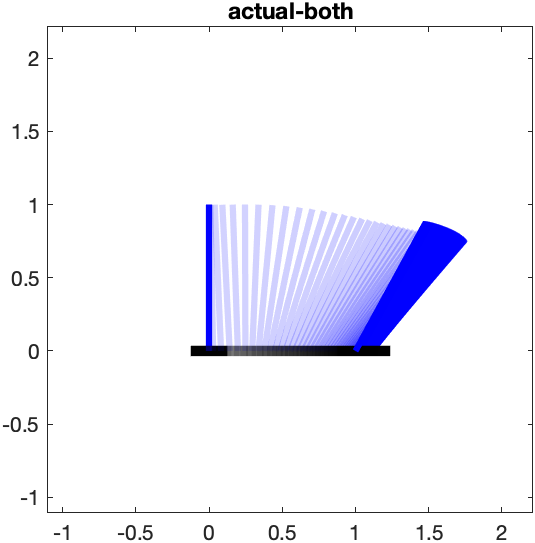
\includegraphics[height=200px]{../matlab/output/p5/mimo_sim_actual-both}
	\caption{Simulation of the actual plant with the controller designed (combined step input)}
	\label{fig:p5:P3_aug:sim:both}
\end{figure}

The result looks pretty good, except the undershoot in the rod angle from the coupling effects from the base motion. The final steady-state for both final position and final rod angle looks decent.

%%%%%%%%%%%%%%%%
%%%%% Ex 6 %%%%%
%%%%%%%%%%%%%%%%
\newpage
\section{Problem P6: Use of state-space methods to control the MIMO aiming system}
%\vspace{5pt}
% --- ANS (a) --- %
\subsection{(a) MIMO one-rod aiming system \label{ans:P6-a}}

% --- ANS (b) --- %
\subsection{(b) MIMO two-rod aiming system \label{ans:P6-b}}

%%%%%%%%%%%%%%%%%%%%%%%%%%%%%%%%%%%%%%%%%%%%%%%%%%%%%%%%%%%%%%%%%%%%%%%%%%%%%%%%
%% ************************************************************************** %%
%% *                      TODO [Remove For Final Copy!]                     * %%
%% ************************************************************************** %%
%%%%%%%%%%%%%%%%%%%%%%%%%%%%%%%%%%%%%%%%%%%%%%%%%%%%%%%%%%%%%%%%%%%%%%%%%%%%%%%%
%\printlistoftodos

%%%%%%%%%%%%%%%%%%%%%%%%%%%%%%%%%%%%%%%%%%%%%%%%%%%%%%%%%%%%%%%%%%%%%%%%%%%%%%%%
%% ************************************************************************** %%
%% *                                Glossary                                * %%
%% ************************************************************************** %%
%%%%%%%%%%%%%%%%%%%%%%%%%%%%%%%%%%%%%%%%%%%%%%%%%%%%%%%%%%%%%%%%%%%%%%%%%%%%%%%%
\clearpage
\printglossaries

%%%%%%%%%%%%%%%%%%%%%%%%%%%%%%%%%%%%%%%%%%%%%%%%%%%%%%%%%%%%%%%%%%%%%%%%%%%%%%%%
%% ************************************************************************** %%
%% *                               References                               * %%
%% ************************************************************************** %%
%%%%%%%%%%%%%%%%%%%%%%%%%%%%%%%%%%%%%%%%%%%%%%%%%%%%%%%%%%%%%%%%%%%%%%%%%%%%%%%%

% \printbibliography[heading=none]

%%%%%%%%%%%%%%%%%%%%%%%%%%%%%%%%%%%%%%%%%%%%%%%%%%%%%%%%%%%%%%%%%%%%%%%%%%%%%%%%
%% ************************************************************************** %%
%% *                               Appendices                               * %%
%% ************************************************************************** %%
%%%%%%%%%%%%%%%%%%%%%%%%%%%%%%%%%%%%%%%%%%%%%%%%%%%%%%%%%%%%%%%%%%%%%%%%%%%%%%%%
% appendices use section and subsection numbering
%\clearpage
\appendix
\begin{appendices}
% INPUT UR APPENDIX
%\section{Code for Main}
%\lstinputlisting[language=MATLAB, caption=Main Lab Contents, label=code:main]{../matlab/main_p3p4.m}
%
%
%\section{Code for Helper Class}
%\lstinputlisting[language=MATLAB, caption=Helper and commonly used functions by main, label=code:helper]{../matlab/helper.m}

\end{appendices}

\end{document}


